By Hao Xu.
\subsection{签名}
假设签名者Alice有一个公钥的集合$\{P_{i,j}|0 \leq i \leq n-1 , 0 \leq j \leq m_i-1\}$。其中$n$是环的个数,$m_i$是第\(i\)个环的元素个数。Alice希望用\(n\)个key $\{P_{i,a_i}\}$对应的私钥$x_i$去产生一个环签名,其中$a_i$由Alice挑选,作为环的起点,验证者并不知道。\par
Alice签名步骤如下:
\begin{enumerate}
	\item 对消息\(m\)进行哈希得到\(M\),并统计所有公钥。
	\item 对于每一个$0 \leq i \leq n-1$,
	\begin{enumerate}
		\item 随机选择一个标量$k_i$.
		\item 设置$e_{i,a_i+1}=H(M||k_iG||i||a_i)$.
		\item 对于每个$a_i+1 \leq j < m_i-1$,随机选取$s_{i,j}$的值,并计算
		\begin{equation*}
		e_{i,j+1}=H(M||s_{i,j}G-e_{i,j}P_{i,j}||i||j).
		\end{equation*}
	\end{enumerate}\par
	至此计算了每个环中编号大于$a_i$的所有点的\(e\)值和\(s\)值。
\item 对于每个环,选取编号最大的点的\(s\)和\(e\)值,分别为$s_{i,m_i-1}$和$e_{i,m_i-1}$。并计算$e_0$,公式如下:
\begin{equation*}
e_0=H(s_{0,m_0-1}G-e_{0,m_0-1}P_{0,0}||\dots||s_{n-1,m_{n-1}-1}G-e_{n-1,m_{n-1}-1}P_{n-1,m_{n-1}-1})
\end{equation*}\par 
由公式可知,$e_0$值取决于\(n\)个点的\(s\)和\(e\)的值。
\item 对每个$0 \leq i \leq n-1$:
\begin{enumerate}
	\item 对于每一个$0 \leq j < a_i-1 $,随机选择$s_{i,j}$的值,并计算
			\begin{equation*}
				e_{i,j+1}=H(M||s_{i,j}G-e_{i,j}P_{i,j}||i||j).
			\end{equation*}
			其中$e_{i,0}$即为$e_0$。这一步计算了每个环中编号小于$a_i$的所有点的\(e\)值和\(s\)值,以及$a_i$的\(e\)值。
		\item 计算$a_i$的\(s\)值如下:$s_{i,a_i}=k_i+x_ie_{i,a_i}$.
\end{enumerate}
\end{enumerate}\par 
最后生成的环签名如下:
\begin{equation*}
\sigma =\{e_0, s_{i,j} :0 \leq i \leq n, 0 \leq j \leq m_i\}
\end{equation*}

\subsection{验签}
假设验证者的已知信息为消息\(m\),公钥集$\{P_{i,j}|0 \leq i \leq n-1 , 0 \leq j \leq m_i-1\}$和签名$\sigma$。\par 
验证者验证签名过程如下:\par 
\begin{enumerate}
	\item 对消息\(m\)进行哈希得到\(M\).
	\item 对于每个$0 \leq i \leq n-1$和$0 \leq j \leq m_j-1$,计算$R_{i,j+1}=s_{i,j}G+e_{i,j}P_{i,j}$和$e_{i,j+1}=H(M||R_{i,j+1}||i||j)$.
	\item 计算$e'_0=H(R_{0,m_0-1}||\dots||R_{n-1,m_{n-1}-1})$。并比较$e'_0 \overset{?}{=}e_0$,若相等,则验证通过。
\end{enumerate}
以上签名过程的示意图如\figurename~\ref{fig-borromean-sig}.
\begin{figure}[!htbp]
	\centering
	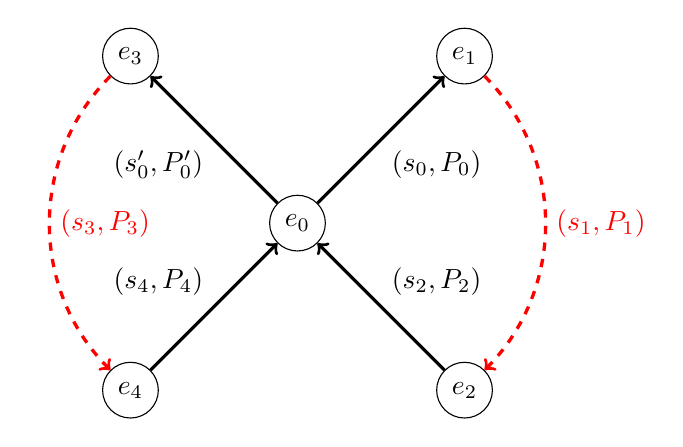
\begin{tikzpicture}[auto,bend angle=45,node distance=3cm,
		place/.style={circle,draw},marrow/.style={->,very thick}]
		\node[place] (e0) {\(e_0\)};
		\node[place] (e1) [above right of=e0] {\(e_1\)};
		\node[place] (e2) [below right of=e0] {\(e_2\)};
		\node[place] (e3) [above left of=e0] {\(e_3\)};
		\node[place] (e4) [below left of=e0] {\(e_4\)};

		% connection
		\draw [marrow] (e0) to node [swap] {\( (s_0,P_0)\)} (e1);
		\draw [marrow,dashed,red] (e1) to [bend left] node {\( (s_1,P_1)\)} (e2);
		\draw [marrow] (e2) to node  [swap]{\( (s_2,P_2)\)} (e0);

		\draw [marrow] (e0) to node {\( (s_0',P_0')\)} (e3);
		\draw [marrow,dashed,red] (e3) to [bend right] node {\( (s_3,P_3)\)} (e4);
		\draw [marrow] (e4) to node {\( (s_4,P_4)\)} (e0);
	\end{tikzpicture}
	\caption{A Borromean ring signature for \( (P_0|P_1|P_2)\&(P_0'|P_3|P_4)\)}\label{fig-borromean-sig}
\end{figure}
